\documentclass{standalone}
\usepackage{amsmath}
\usepackage{tikz-cd}
\usetikzlibrary{positioning}
\begin{document}

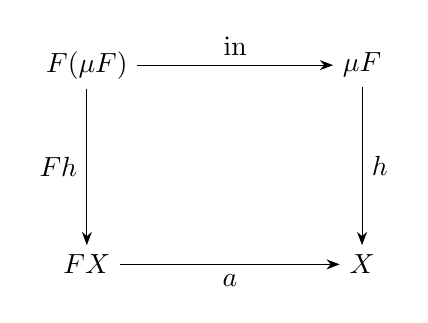
\begin{tikzpicture}[>=Stealth, node distance=2cm]
  \matrix (m) [matrix of nodes,
               row sep=2cm,
               column sep=2.5cm,
               nodes={anchor=center}] {
    $F(\mu F)$ & $\mu F$ \\
    $F X$      & $X$     \\
  };

  % Nodes in matrix
  \draw[->] (m-1-1) -- (m-2-1) node[midway,left] {$Fh$};
  \draw[->] (m-2-1) -- (m-2-2) node[midway,below] {$a$};
  \draw[->] (m-1-1) -- (m-1-2) node[midway,above] {in};
  \draw[->] (m-1-2) -- (m-2-2) node[midway,right] {$h$};
\end{tikzpicture}

\end{document}
